\documentclass{article}
\usepackage{graphicx}
\usepackage{float}
\floatstyle{boxed} 
\restylefloat{figure}

\title{Computer Design Laboratory Project}
\author{Levi Balling \and Robert Christensen \and T. James Lewis}
\date{December 2011}
\begin{document}
\maketitle
\pagebreak


\begin{abstract}
	We implemented a 16-bit computer with VGA graphics for output, a NES gamepad used for input, and an RS-232 type serial controller used for communications. The software developed for this computer is a maze game in which players maneuver through a maze trying to reach the exit first. The players play on two machines, each with its own monitor, and communication between the machines is over a serial connection.
\end{abstract}

\section{Introduction}
Our goal was to produce a computer platform capable of running a game with the following features: Levels that were larger than the screen and which scrolled when the player moved near an edge, two players on different machines playing against each other with interaction, and using an NES game pad for user input. To allow large levels we needed a mechanism to store the level information compactly, as the block memory we were using was not large enough to store bitmaps as large as the levels. To allow linked play between two machines we needed to implement some form of communication between them. To use NES game pads for input we needed to research how they transmitted the input to the machine and device and interface to work with them.

The overall organization of the system can be seen in figure \ref{oo} we have a main memory module which is a two port block memory that both the CPU and VGA controller have access to. The Gamepad Controller module is connected to the CPU, and the Serial Controller is also connected to the CPU. The VGA Controller has pin-outs to the VGA port on the board, the gamepad controller has pin-outs to the gamepad, and the serial controller has pin-outs to the serial port.

\begin{figure}[h!]
	\centering
	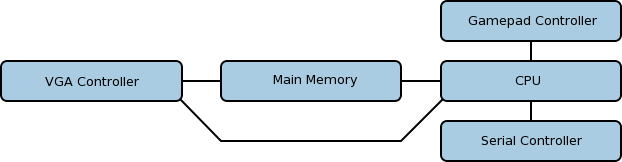
\includegraphics[width = 1\textwidth]{OverallOrganization.png}
	\caption{Overall Organization}
	\label{oo}
\end{figure}

A lot of the work required to render a game level to the screen is taken care of by hardware in the VGA Controller. There is a section in main memory where the map to be drawn is stored as a series of tile numbers, the VGA Controller reads these tile numbers from main memory, and for each tile number looks in its internal memory for the pixel map corresponding to the tile number and draws the pixels in the right section of the screen. The CPU has two registers which are directly wired to the VGA controller that tell the VGA controller where to look in main memory for the tile to be placed at the upper left corner of the screen and also what the row offset is. This makes the code for scrolling the screen to show only a section of the entire map as simple as setting the address for the upper left corner of the screen to a different location, rather than having the CPU rewrite the entire map area with new data to scroll.

\section{CPU Design}



\section{VGA Controller}
We used a 640$\times$480 VGA display with a 25 Mhz clock. This was done with the use of sync signals, and memory manipulation. The 640$\times$480 pixel display was broken up into 20$\times$15 blocks on the screen. This allowed us to conserve memory and still have meaningful graphics.  The graphics used 3 bit colors, and we were able to display 8 different colors. Using different patterns with these colors we were able to display 14 32$\times$32 pixel images.

\subsection{Sync Signals}
For the monitor to recognize which pixel it is on, it needs to receive 2 signals, Vsync and Hsync.  These signals will be sent on specific patterns because it generates different resolutions. We used a 25 Mhz clock input to generate the different signals. While we generated the signals, we kept track of which columns and rows the VGA was on. We used the columns and rows to find out which group of pixels it was on.  As well as the individual sub pixels that it is on in the 32$\times$32 block of pixels.

\subsection{VGA Memory}
We had organized our memory to have 2 separate memory blocks.  Main memory used a 2 port 14 bit addressable memory block containing 16 bit words. Our VGA memory contained a 14 bit addressable single port containing 9 bit words.  One of the 9 bit words contains 3 separate pixels.   We used each memory value twice, so we display the value of 3 bits for 2 pixels. We have an input to the bit generator where the starting address and row size of the image are.  This way we can fetch the entire cell in main memory that we would like to display.

\begin{figure}[h!]
	\centering
	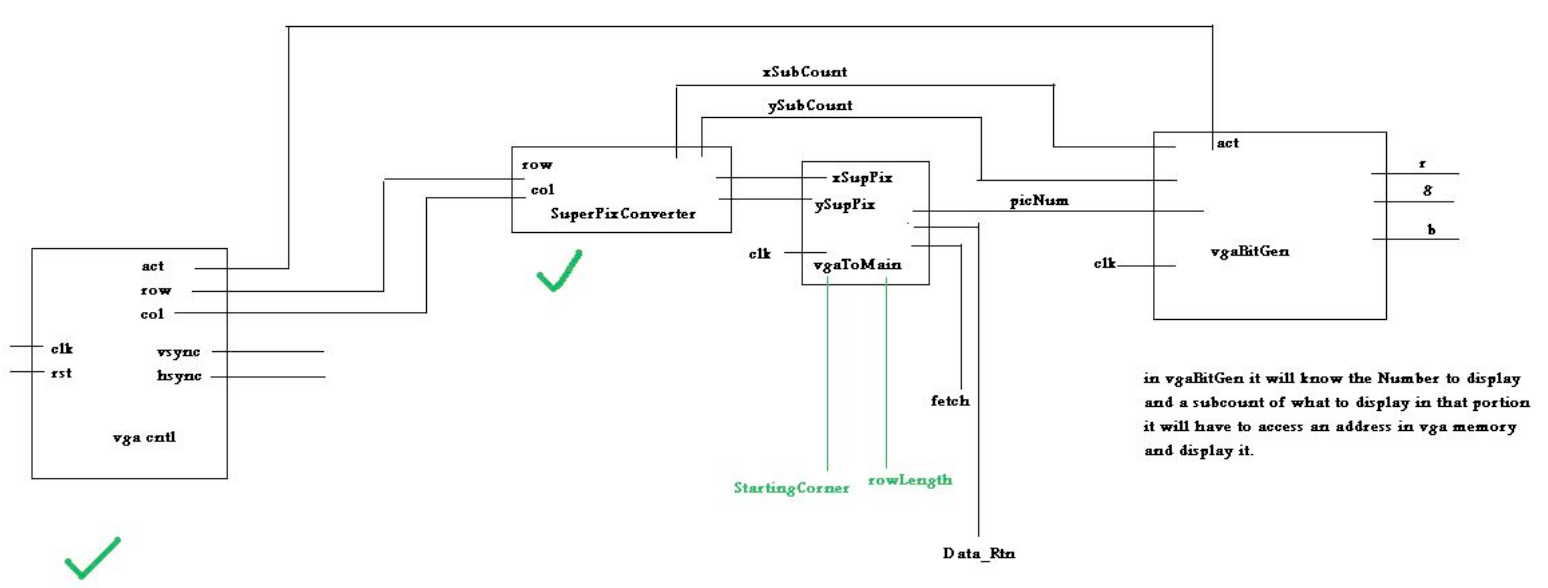
\includegraphics[width = 1\textwidth]{VGAdiagram.png}
	\label{vga}
\end{figure}

In main memory we have an area specially set aside just for our levels.  These memory words contain a number from 0 to 14.  These words are related to the image that we want to display on that portion of the screen.  The VGA controller will read from main memory, find out what should be displayed on the block of the screen based on what number it is, and then go and display all of the values on the screen based on the number from 0 to 14.  From that number it will find the correct address in VGA memory that it should display for that pixel. 
 

\section{NES Controller}
For our game system we used a classic Nintendo Controller (figure \ref{nes}). This device required 5 lines to the controller: Power, Ground, Latch, Pulse, and Data.  The timing input for our controller was 25 Mhz, the module throttle was around 1Mhz and we achieved around 100 samples per second. This allowed us to read the input, detect whether the values were high or low and store it in a register. 

\begin{figure}[h!]
	\centering
	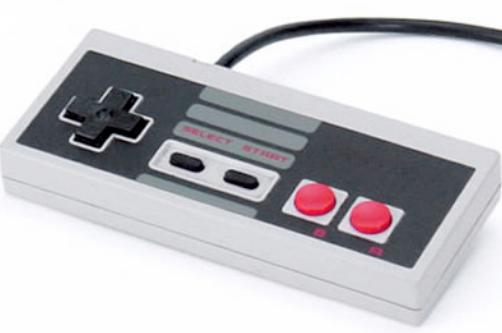
\includegraphics[width = .5\textwidth]{nescontroller.png}
	\label{nes}
\end{figure}

\section{Serial Controller}

\section{Assembler}

\begin{figure}[h!]
	\centering
	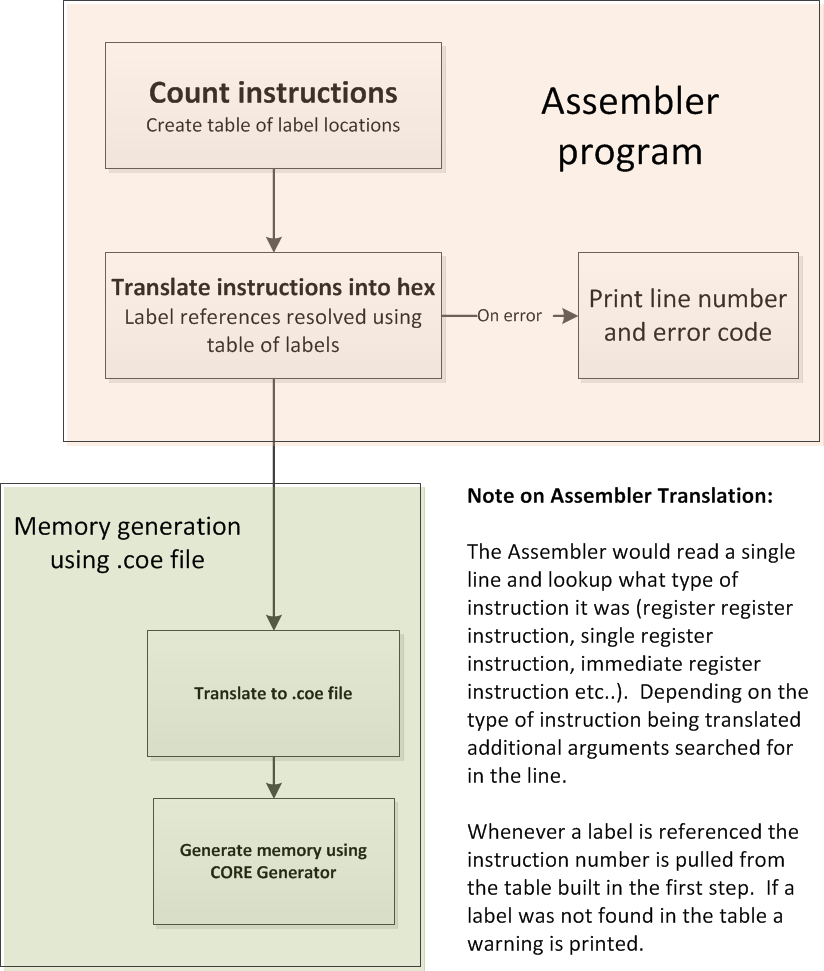
\includegraphics[width = 3in]{assembler_diagram.png}
	\caption{Tool chain for assembling and loading a program}
	\label{fig:assembler}
\end{figure}

The assembler architecture was heavily influenced by an assignment given in a hardware design lab at a different university.\cite{Assembler}  The assignment provided suggestions for writing a simple assembler using the C programming language.  These hints where considered in the development of the assembler that was used in this project.

The assembler was written using the C++, as opposed to C, in order to use the standard template library.  A map was used to store the table of labels and their locations in code.  The program was written to be compiled using the g++ compiler.

Figure \ref{fig:assembler} shows how the assembler tool chain works.  The assembly file is scanned twice.  The first pass fills the table of label locations.  In order to do this each instruction must be counted.  Pseudo code instructions are counted as however many assembly instructions it will take in the output.  By linearly counting the number of previous memory locations used each label can be associated with the correct memory location in the output.

The second pass though the input translates each line into the appropriate hex value for the instruction.  The instruction could be a pseudo instruction, which is split into multiple assembly instruction; a fill value, where the assembler will place a specific value at that memory location; or an assembly instruction.  The only pseudo instruction used in the current implementation was used to load label locations into a specific register.  Since a single move instruction only load 8 bits into a register, and only the assembler knows the value of 16 bit label reference, this pseudo instruction was created.  Whenever a label reference is found in any instruction, the value of the label is pulled from the table and substituted appropriately.

When an assembly instruction is found, the assembler does a look-up for what type of instruction is being used.  Seven unique instruction types were used in the CPU implementation.  Doing a look-up would tell the assembler how many registers and immediate value to expect following the instruction, and how to pack the bits for the output.  Anytime the program found something unexpected it printed where the error was encountered and stopped the assembly process.  

Compiler options were created to print extra information to help debug assembly programs for the CPU.  If the assembler was built using the special debug flags additional information was reported to the user.  As bugs were found in assembly programs the assembler was modified to help detect future occurrences of the error.  However, the assembler was desired to be robust and accepting of programmer desired, so warning were issued for common problems rather than errors.

\section{Software}

\begin{figure}[h!]
	\centering
	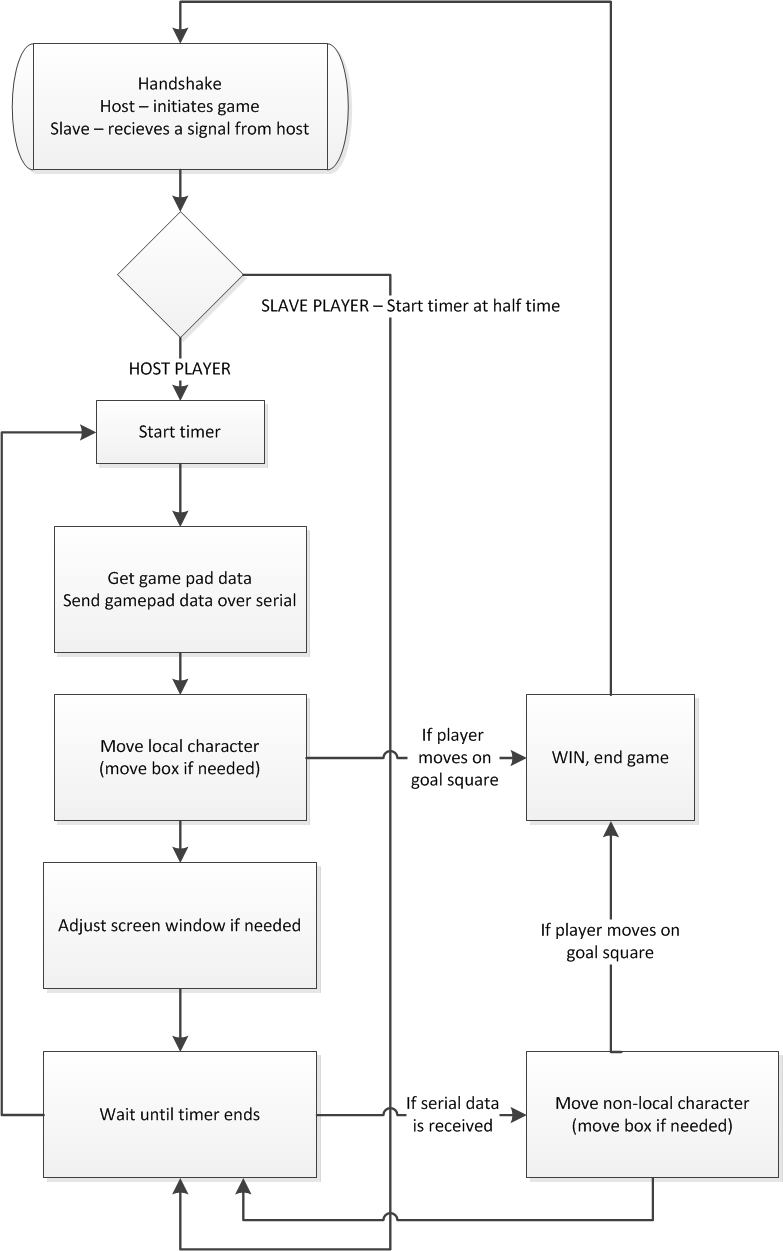
\includegraphics[width = 3in]{game.png}
	\caption{Progression of states in multiplier maze game}
	\label{fig:assembler}
\end{figure}

A coding standard was developed for the CPU.  The following were explicitly defined in the standard: save registers, temporary registers, register use for passing information to methods, stack usage, global variables, and naming of labels.  The standard was designed to increase readability and consistency of assembly code.  This standard was found to increase development speed and speed of bug fixes.

The game that was developed for the CPU was a simple multiplayer maze puzzle game.  The goal of the game is to move the player to a goal location.  The game supports movable blocks, which could be used to cover lava squares to create a bridge, or the blocks could be used to block the path of the opposing player.  The movable blocks created a variety of entertaining gameplay.

The architecture of the multiplayer game was designed to be simple.  No error correction or special timing synchronization was added.  This architecture made the software easy to write to allow for either single or multiplayer gameplay using the same excitable.  The basic flow of the game is shown in fig. \ref{fig:assembler}.

When the game was played as a multiplayer game, one player would move and send the its movement to the other device.  Following its movement it would enter a waiting state for 250ms.  If data was received on the serial line the non-local player would move.  The movement of each player was offset by 125ms.  By offsetting each player movement, no turn priority would need to be programmed, since only one player will be moving at a given time.  This design decision was made with the assumption that a game would not last very long, both boards run at nearly the same clock speed, and all data sent across the serial line would be received by the other board.

Multiplayer functionality was developed using this method.  However, the two games would quickly become unsynchronized.  It was found that a significant number of writes to the serial line were never received by the other board.  The assumption that all data sent across the serial line would be received by the other board was not true, so this architecture would not work for multiplayer.

A redesign of the multiplayer portion of the code was started that would detect and resend lost packets was started.  The design of the patch was developed, but the programming was not finished due to lack of time.

\section{System Integration}

\section{Conclusions and Further Work}

All CPU features that were planned to be implemented were implemented and demoed.  NES game pad input and VGA output worked extremely well.  Serial communication was also developed.  It was not completely understood if the problem was in the software or hardware, however, the software should have had some ability to do error correction for lost packets.

The VGA system of the computer was designed to work very well with large two-dimensional maps.  Adjusting what portion of a map is being displayed on the VGA is a single CPU instruction.  This simplified the development of the maze game significantly.

Interfaces with peripheral was done by polling the peripheral for information.  A CPU instruction was executed to grab information from the game pad and serial device.  Future programs for this device would need to accommodate for this.

A software error correction could be developed to request information expected but not received.  This would improve the usability of serial communication.  More investigation is needed to know if the problems seen in the serial communication could have been improved in hardware.

The tools for loading an assembled program onto the device was very slow.  Since CORE Generator was used to create the memory for the CPU it was non-trivial to modify the memory without regenerating the memory and resynthesizing the entire CPU.  This would take several minutes.  This caused frustration when only minor changes were made to a program because it could not be tested until the memory and CPU was regenerated.  The memory would need to be modified to make it capable of changing memory initialization without regenerating everything.

\section{Individual Contributions}

\subsection{Levi Balling}

\subsection{Robert Christensen}

Assisted in developing the ALU component of the CPU.  Developed main memory and VGA memory modules using CORE Gen, and verified memories were correctly initialized.

Developed the assembly tool chain.  Verified the correctness of CPU components by using programs written in assembly.  Architect and lead programmer of the maze game.

\subsection{T. James Lewis}

\begin{thebibliography}{99}

\bibitem{Serial} Serial Interface (RS-232) \texttt{fpga4fun.com/SerialInterface.html}

\bibitem{Assembler}ENEE 646: Digital Computer Design, Fall 2011 \texttt{http://www.ece.umd.edu/class/enee646/p1.pdf}

\end{thebibliography}
\end{document}
